\chapter{Method of Moments and M-Estimation}
\label{ch:mom-mestimation}

\begin{chaptergoals}
\begin{itemize}[nosep]
\item The method of moments: match the sample mean, mean square and so on to their population versions, and solve for the parameter. Older than maximum likelihood, often the same answer, always a formula.
\item Its asymptotic variance, by the delta method, and why it is never smaller than the maximum likelihood estimator's.
\item M-estimation: the general recipe behind both. Pick a loss whose expected value is smallest at the quantity you want, average the loss over the data, minimize. The sample mean, the median, every quantile and the MLE are all instances.
\item The asymptotic variance of an M-estimator, $J^{-1}KJ^{-1}$, by the argument of \cref{ch:mle-properties} with two matrices in place of one. The Laplace median has asymptotic variance $1$, as \cref{ch:mle-properties} promised.
\item Robustness: when the data have heavy tails or a few wild values, the median and Huber's estimator keep working and the mean does not. The Cauchy distribution, for which the sample mean never settles down.
\end{itemize}
\Cref{ch:mle-properties} finished maximum likelihood. This chapter puts the two other estimation recipes beside it and shows all three are one idea.
\end{chaptergoals}

\section{Three recipes, one idea}
\label{sec:mom-idea}

Every estimator in Part III was pulled out of the air: the sample proportion for $p$, the sample mean for $\mu$, $1/\bar{T}_n$ for the subway rate.
Each looked obvious, and \cref{ch:likelihood} showed that maximum likelihood produces each of them from a principle.
This chapter gives two more principles.
The method of moments is the older and simpler one: write the parameter as a function of the population mean (and mean square, and so on), then replace the population moments by sample moments.
M-estimation is the more general: choose a loss function, average it over the data, minimize.
Maximum likelihood is M-estimation with the negative log-likelihood as the loss, and the method of moments is M-estimation with a squared-distance loss, so this chapter also explains what the three have in common and why the limit theorems of \cref{ch:mle-properties} apply to all of them.

\section{The method of moments}
\label{sec:mom}

\recall{The Law of Large Numbers (\cref{thm:wlln}): for i.i.d.\ $\Xton$ and a function $h$ with $\var(h(X)) < \infty$, $\frac1n\sum_{i=1}^n h(X_i) \convp \E[h(X)]$.}

The $k$th \textbf{moment} of a distribution $\Pr_\theta$ is $m_k(\theta) = \E_\theta[X^k]$: the mean for $k = 1$, the mean square for $k = 2$.
Its sample version is $\hat{m}_k = \frac1n\sum_{i=1}^n X_i^k$, and by the LLN (with $h(x) = x^k$, which needs $\E[X^{2k}] < \infty$), $\hat{m}_k \convp m_k(\theta^*)$.
So the sample moments are consistent estimators of the population moments.
The method of moments turns that into an estimator of $\theta$ by inverting the map from parameters to moments.

\begin{definition}[Method of moments estimator]
\label{def:mom}
Let $(E, (\Pr_\theta)_{\theta \in \Theta})$ be a model with $E \subset \real$ and $\Theta \subset \real^d$, and let $M(\theta) = (m_1(\theta), \ldots, m_d(\theta))$ be its \textbf{moment map}, assumed one-to-one.
The \textbf{method of moments estimator} is
\[
\hat{\theta}_n^{\text{MM}} = M^{-1}(\hat{m}_1, \ldots, \hat{m}_d),
\]
the parameter whose first $d$ population moments equal the first $d$ sample moments, provided one exists.
\end{definition}

\begin{inwords}
\textbf{In words.} A model with $d$ unknowns needs $d$ equations. The method of moments writes down $d$ of them: the population mean equals the sample mean, the population mean square equals the sample mean square, and so on up to $d$. Solve for the $d$ unknowns. The hope is that $d$ moments pin down $d$ parameters, which is what `one-to-one' asks of the moment map.
\par\smallskip
\textbf{For the kiss data.} One parameter, one equation: $m_1(p) = \E_p[R] = p$, so $M(p) = p$, $M^{-1}$ is the identity, and $\hat{p}^{\text{MM}} = \hat{m}_1 = \bar{R}_n = 0.645$. For a proportion the method of moments is the sample proportion, as every method so far has been.
\end{inwords}

\Cref{fig:mommatching} draws the definition for two families.
On the right, the exponential family has one parameter and the moment map $m_1(\lambda) = 1/\lambda$ is a curve.
Reading it backwards from the subway's sample mean of $6.23$ minutes gives $\hat{\lambda} = 1/6.23 = 0.1605$, the same estimate as maximum likelihood.
On the left, the Gaussian family has two parameters and the moment map sends $(\mu, \sigma^2)$ to $(m_1, m_2) = (\mu, \sigma^2 + \mu^2)$.
The parameters with the sample's $\hat{m}_1 = 70.9$ lie on a vertical line, those with its $\hat{m}_2 = 5{,}210$ on a curve, and the two cross once, at the estimate: $\hat{\mu} = 70.9$ minutes and $\widehat{\sigma^2} = 184.1$ for the $272$ Old Faithful waits of \cref{ch:likelihood}.

\begin{figure}[htbp]
\centering
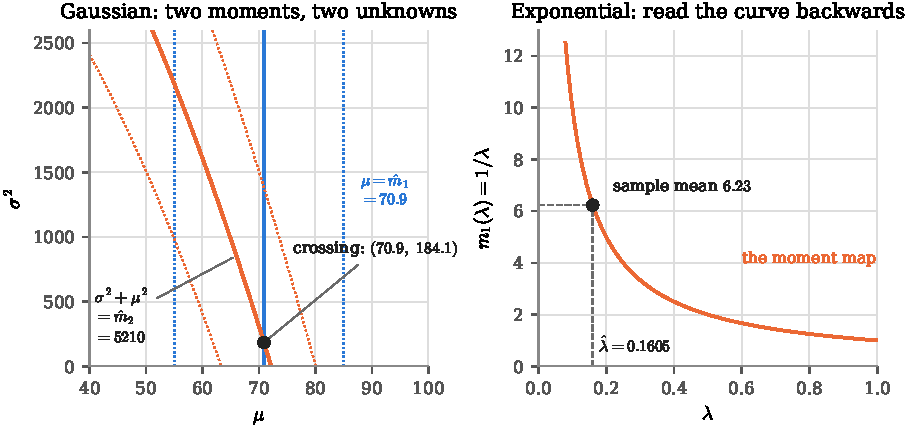
\includegraphics[width=\textwidth]{fig_mom_matching}
\caption{Left: the Gaussian moment map, with the parameters having the Old Faithful sample mean (blue) and sample mean square (orange) crossing at the estimate; dotted: other values of $m_1$ and $m_2$. Right: the exponential moment map $m_1 = 1/\lambda$, read backwards from the subway sample mean.}
\label{fig:mommatching}
\end{figure}

\begin{worked}[method of moments for the standard families]
\begin{itemize}
\item \textbf{Bernoulli.} $m_1(p) = p$, so $\hat{p} = \bar{X}_n$.
\item \textbf{Poisson.} $m_1(\lambda) = \lambda$, so $\hat{\lambda} = \bar{X}_n$. For the siblings data with $X - 1 \sim \Pois(\lambda)$, $m_1 = \lambda + 1$ and $\hat{\lambda} = \bar{X}_n - 1 = 1.0$, which is how \cref{ch:models} fitted it in the first place.
\item \textbf{Exponential.} $m_1(\lambda) = 1/\lambda$, so $\hat{\lambda} = 1/\bar{X}_n$.
\item \textbf{Gaussian.} $m_1 = \mu$ and $m_2 = \sigma^2 + \mu^2$. Solving, $\hat{\mu} = \hat{m}_1 = \bar{X}_n$ and $\widehat{\sigma^2} = \hat{m}_2 - \hat{m}_1^2 = \frac1n\sum_i X_i^2 - \bar{X}_n^2 = \frac1n\sum_i (X_i - \bar{X}_n)^2$: the divide-by-$n$ variance, which is the MLE as well.
\item \textbf{Uniform.} For $\Unif([0, \theta])$, $m_1 = \theta/2$, so $\hat{\theta}^{\text{MM}} = 2\bar{X}_n$. This one differs from the MLE $\max_i X_i$, and it can be absurd: for the five observations of \cref{fig:uniformlik}, with mean $4.84$, it gives $9.68$, which is fine, but a sample of $1, 1, 1, 1, 7.6$ gives $4.64$, below an observation the model then calls impossible.
\end{itemize}
For the Bernoulli, Poisson, exponential and Gaussian families the method of moments is the maximum likelihood estimator; for the uniform it is not, and for the Laplace model of \cref{ex:lik-laplace} the method of moments gives the sample mean while maximum likelihood gives the median.
The agreement for the first four is not a coincidence, and \cref{ch:exp-families} explains it: in an exponential family the likelihood equations match the moments of the sufficient statistics, which for these four families are the moments of $X$ itself.
\end{worked}

\begin{bridge}[the method of moments is how your first statistics course estimated everything]
An introductory course estimates a population mean by the sample mean, a variance by the sample variance, a proportion by the sample proportion, a correlation by the sample correlation.
Each of those is the method of moments: a population quantity written in terms of moments, with sample moments plugged in.
Karl Pearson named the method in 1894, before maximum likelihood existed, and it is still the first thing to try when a model's likelihood is awkward, since solving $d$ polynomial equations is usually easier than maximizing a function.
What the introductory course did not say is how precise the plug-in is, which is the next section.
\end{bridge}

\subsection{Asymptotic variance of the method of moments}
\label{sec:mom-variance}

\recall{The delta method (\cref{thm:delta}): if $\sqrt{n}(Z_n - \theta) \convd \Gauss(0, \sigma^2)$ and $g$ is continuously differentiable at $\theta$, then $\sqrt{n}(g(Z_n) - g(\theta)) \convd \Gauss(0, g'(\theta)^2\sigma^2)$. The Central Limit Theorem (\cref{thm:clt}): for i.i.d.\ $Y_i$ with mean $m$ and variance $s^2 < \infty$, $\sqrt{n}(\bar{Y}_n - m) \convd \Gauss(0, s^2)$. Slutsky's theorem (\cref{thm:slutsky}): if $X_n \convd X$ and $Y_n \convp y$, then $X_n Y_n \convd yX$ and, for $y \neq 0$, $X_n/Y_n \convd X/y$. Vector versions (the vector-versions remark of \cref{ch:limit-tools}): for i.i.d.\ vectors $V_i$ with mean $m$ and finite covariance matrix $\Sigma$, $\sqrt{n}(\bar{V}_n - m) \convd \Gauss_d(0, \Sigma)$, a Gaussian vector, meaning that every linear combination $a^\top Z$ of its coordinates is Gaussian, with variance $a^\top\Sigma a$; and for $g: \real^d \to \real^d$ continuously differentiable at $m$ with Jacobian matrix $G$ (row $j$ is the gradient of the $j$th coordinate of $g$), $\sqrt{n}(g(\bar{V}_n) - g(m)) \convd \Gauss_d(0, G\Sigma G^\top)$.}

A method of moments estimator is a function, $M^{-1}$, of sample moments, and sample moments are averages.
So the CLT gives the limit of the moments and the delta method carries it through $M^{-1}$.

\begin{theorem}[Asymptotic normality of the method of moments]
\label{thm:mom-normal}
Suppose $\Xton \iid \Pr_{\theta^*}$, the moment map $M$ is one-to-one, its image $M(\Theta)$ contains a neighborhood of $M(\theta^*)$ (so that the estimator exists for sample moments near the population ones), $M^{-1}$ is continuously differentiable at $M(\theta^*)$, and $\E_{\theta^*}[X^{2d}] < \infty$.
Let $\Sigma(\theta^*)$ be the $d \times d$ covariance matrix of the vector $(X, X^2, \ldots, X^d)$ under $\Pr_{\theta^*}$, and $\nabla M^{-1}$ the Jacobian matrix of $M^{-1}$ at $M(\theta^*)$: the $d \times d$ matrix whose row $j$ is the gradient of the $j$th coordinate of $M^{-1}$ (the transpose of the matrix in the vector-versions remark of \cref{ch:limit-tools}, which puts the coordinates in columns).
Then
\[
\sqrt{n}\,\big(\hat{\theta}_n^{\text{MM}} - \theta^*\big) \convd \Gauss_d\big(0, \Gamma(\theta^*)\big), \qquad \Gamma(\theta^*) = \nabla M^{-1}\,\Sigma(\theta^*)\,(\nabla M^{-1})^\top.
\]
For $d = 1$: $\Gamma = \big((M^{-1})'(m_1)\big)^2 \var_{\theta^*}(X)$.
\end{theorem}

\optionalproof{The vector of sample moments is an average of i.i.d.\ vectors, so the multivariate CLT gives $\sqrt{n}(\hat{m} - M(\theta^*)) \convd \Gauss_d(0, \Sigma)$. The estimator is $M^{-1}(\hat{m})$, and the multivariate delta method pushes the Gaussian through $M^{-1}$: the covariance gets multiplied by the derivative matrix on both sides.}
\begin{proof}
The $i$th observation contributes the vector $(X_i, X_i^2, \ldots, X_i^d)$; these vectors are i.i.d.\ with mean $M(\theta^*)$ and covariance $\Sigma(\theta^*)$, finite by the moment condition, and $\hat{m} = (\hat{m}_1, \ldots, \hat{m}_d)$ is their average.
The multivariate CLT of the recall gives $\sqrt{n}(\hat{m} - M(\theta^*)) \convd \Gauss_d(0, \Sigma(\theta^*))$.
For $d = 1$ the delta method applied to $g = M^{-1}$ finishes the proof.
For general $d$, the multivariate delta method is the same argument coordinate by coordinate: the mean value theorem writes $M^{-1}(\hat{m}) - M^{-1}(M(\theta^*))$ as a matrix of derivatives, evaluated at in-between points that converge to $M(\theta^*)$, times $\hat{m} - M(\theta^*)$; the derivative matrix converges in probability to $\nabla M^{-1}$ by continuity, and Slutsky's theorem (\cref{thm:slutsky}) multiplies it into the Gaussian limit.
A matrix $A$ times a Gaussian vector $Z$ with covariance $\Sigma$ is Gaussian with covariance $A\Sigma A^\top$: each linear combination $a^\top AZ = (A^\top a)^\top Z$ is Gaussian with variance $a^\top A \Sigma A^\top a$, and when $A$ is invertible, the linear-map rule of the Toolkit \toolkit{sec:math-gaussquad} shows that $AZ$ is $\Gauss_d(0, A\Sigma A^\top)$ in the sense defined there.
\end{proof}

\begin{worked}[the exponential rate, both ways]
For $\Expo(\lambda)$, $M(\lambda) = 1/\lambda$, $M^{-1}(m) = 1/m$ and $(M^{-1})'(m) = -1/m^2$, which at $m = 1/\lambda$ is $-\lambda^2$.
With $\var(X) = 1/\lambda^2$, the theorem gives asymptotic variance $\lambda^4 \cdot \lambda^{-2} = \lambda^2$: the same as the maximum likelihood estimator's $1/I(\lambda) = \lambda^2$ from \cref{ch:mle-properties}, as it must be, since the two estimators are the same function of the data.
For the subway, standard error $\hat{\lambda}/\sqrt{n} = 0.020$ once more.
\end{worked}

\begin{sanitycheck}[Could a different moment do better?]
The Poisson model has $m_1 = \lambda$, and also $m_2 = \lambda + \lambda^2$.
Nothing in the definition says you must use the first moment; you could match the second instead, solving $\hat{m}_2 = \lambda + \lambda^2$ for $\lambda = \big(-1 + \sqrt{1 + 4\hat{m}_2}\big)/2$.
Is that any better?
The theorem says no.
With $g(m) = (-1 + \sqrt{1 + 4m})/2$, $g'(m_2) = 1/(2\lambda + 1)$, and $\var(X^2) = \lambda + 6\lambda^2 + 4\lambda^3$ for a Poisson, so the asymptotic variance is $(\lambda + 6\lambda^2 + 4\lambda^3)/(2\lambda + 1)^2$, which at $\lambda = 1$ is $11/9 = 1.22$ against $\lambda = 1$ for the sample mean.
The second-moment estimator is $22\%$ noisier.
It throws away information by squaring, and an estimator built on higher moments is usually worse than one built on lower ones, since higher sample moments have larger variance (usually, not always: the derivative of $M^{-1}$ matters as much as the variance of the moment).
\end{sanitycheck}

\begin{proposition}[Method of moments is never better than maximum likelihood]
\label{prop:mom-vs-mle}
In a regular model (\cref{sec:mle-regularity}), under the hypotheses of \cref{thm:mom-normal}, the asymptotic variance of the method of moments estimator is at least that of the maximum likelihood estimator: $\Gamma(\theta^*) \geq 1/I(\theta^*)$ for $d = 1$, and in general $\Gamma - I^{-1}$ is positive semidefinite, meaning $a^\top(\Gamma - I^{-1})a \geq 0$ for every vector $a$: no linear combination of the parameters is estimated more precisely by moments than by likelihood.
\end{proposition}

\optionalproof{The delta step of \cref{thm:mom-normal} writes the method of moments estimator as an average plus a negligible term, and the score is an average too. The multivariate CLT makes the pair jointly Gaussian in the limit, their covariance works out to the identity by the same differentiate-under-the-integral step as in Cram\'er--Rao, and a variance is never negative.}
\begin{proof}
Take $d = 1$ first.
Write $T_n = \hat{\theta}_n^{\text{MM}}$ and $c = (M^{-1})'(m_1(\theta^*))$.
The mean value theorem step in the proof of \cref{thm:mom-normal} gives
\[
\sqrt{n}(T_n - \theta^*) = c\,\sqrt{n}(\hat{m}_1 - m_1(\theta^*)) + R_n, \qquad R_n \convp 0,
\]
since the derivative at the in-between point differs from $c$ by a quantity converging to zero in probability, multiplied by a sequence converging in distribution (Slutsky).
So $\sqrt{n}(T_n - \theta^*)$ is, up to $R_n$, the standardized average of the i.i.d.\ variables $U_i = c(X_i - m_1(\theta^*))$.
The score is the average of the i.i.d.\ variables $W_i = \ell'(\theta^*; X_i)$, with mean zero (\cref{prop:score-mean}) and variance $I(\theta^*)$ (\cref{def:fisher}).
Apply the multivariate CLT to the pairs $(U_i, W_i)$: the pair $\big(\sqrt{n}\bar{U}_n, \sqrt{n}\bar{W}_n\big)$ converges to a Gaussian vector $(U, W)$ with $\var(U) = \Gamma$, $\var(W) = I$ and
\begin{align*}
\cov(U, W) = \cov(U_1, W_1) &= c\,\E_{\theta^*}\!\big[X\,\ell'(\theta^*; X)\big] = c \int x\,\frac{\partial}{\partial\theta}p_{\theta}(x)\Big|_{\theta^*}\,\mathrm{d}x \\
&= c\,\frac{\mathrm{d}}{\mathrm{d}\theta}m_1(\theta)\Big|_{\theta^*} = c\,M'(\theta^*) = 1,
\end{align*}
where the mean-zero score let us drop $m_1(\theta^*)$, the exchange of derivative and integral is the regularity condition used in \cref{thm:cramer-rao}, and the last step is the inverse function rule $(M^{-1})'(M(\theta^*)) = 1/M'(\theta^*)$.
Adding $R_n$ does not change the limit (Slutsky).
Now $\var(U - W/I) = \Gamma - 2\cdot\frac{1}{I} + \frac{I}{I^2} = \Gamma - \frac1I \geq 0$, which is the claim.

For general $d$ the same steps give a Gaussian vector $(U, W)$ in $\real^{2d}$, with $U$ having covariance $\Gamma$, $W$ the score vector with covariance $I$, and $\cov(U, W) = \nabla M^{-1}\,\nabla M = $ the identity matrix, since the matrix of $\partial m_k/\partial\theta_j$ is the Jacobian $\nabla M$ and the inverse function rule inverts it.
For any vector $a$, $\var\big(a^\top U - a^\top I^{-1}W\big) = a^\top\Gamma a - 2a^\top I^{-1}a + a^\top I^{-1}II^{-1}a = a^\top(\Gamma - I^{-1})a \geq 0$.
\end{proof}

So when maximum likelihood is available, it is at least as precise.
The method of moments is the tool elsewhere: when the likelihood has no tractable maximum (the mixture of \cref{sec:lik-em} is a classic case, and Pearson's 1894 paper fitted a mixture of two Gaussians by matching five moments), or when it is the same estimator anyway and the moment version is easier to compute.

\section{M-estimation}
\label{sec:mest}

Both recipes so far minimized something.
Maximum likelihood minimized $-\frac1n\sum_i\log p_\theta(X_i)$.
The method of moments, for $d = 1$, solves $\hat{m}_1 = m_1(\theta)$, which is where $\frac1n\sum_i(X_i - m_1(\theta))^2$ has zero derivative with respect to $m_1$.
Here is the general pattern.

\begin{definition}[M-estimator]
\label{def:mest}
Let $\Xton$ be i.i.d.\ from a distribution $\Pr$ on $E$, and let $\mu^* \in \mathcal{M} \subset \real^d$ be a quantity attached to $\Pr$ that you want to estimate.
A \textbf{loss function} for $\mu^*$ is a function $\rho: E \times \mathcal{M} \to \real$ with $\E\abs{\rho(X, \mu)} < \infty$ for every $\mu$, such that the \textbf{expected loss}
\[
Q(\mu) = \E\big[\rho(X, \mu)\big]
\]
is smallest at $\mu = \mu^*$, and only there.
The \textbf{M-estimator} of $\mu^*$ is the minimizer of the \textbf{empirical loss},
\[
\hat{\mu}_n = \operatorname*{argmin}_{\mu \in \mathcal{M}} Q_n(\mu), \qquad Q_n(\mu) = \frac1n\sum_{i=1}^n \rho(X_i, \mu).
\]
\end{definition}

\begin{inwords}
\textbf{In words.} You want a number attached to the distribution: its mean, its median, a parameter. Find a loss that charges each observation according to how far it is from a candidate $\mu$, chosen so that the average charge over the whole distribution is smallest at the number you want. You cannot compute that average, but the LLN says the average over the data is close to it, so minimize the data's average instead. No statistical model is needed: the recipe asks only that $Q$ have its minimum at $\mu^*$.
\par\smallskip
\textbf{For the kiss data.} With $\rho(r, \mu) = (r - \mu)^2$, $Q(\mu) = \E[(R - \mu)^2] = \var(R) + (p - \mu)^2$ is smallest at $\mu = p$, and $Q_n(\mu) = \frac1n\sum_i(R_i - \mu)^2$ is smallest at $\bar{R}_n = 0.645$. The sample proportion is an M-estimator for the squared loss, which is its fourth derivation in this book.
\end{inwords}

\begin{worked}[losses and what they estimate]
\begin{itemize}
\item \textbf{Squared loss, $\rho(x, \mu) = (x - \mu)^2$.} $Q(\mu) = \var(X) + (\E[X] - \mu)^2$, minimized at $\mu^* = \E[X]$ (when $\var(X) < \infty$). The M-estimator is the sample mean: for the Old Faithful waits, $Q_n$ is minimized at $70.9$ minutes, the blue dot in \cref{fig:mestlosses}. In $\real^d$, with $\rho = \norm{x - \mu}^2$, it is the vector of sample means.
\item \textbf{Absolute loss, $\rho(x, \mu) = \abs{x - \mu}$.} $Q(\mu) = \E\abs{X - \mu}$ is minimized at a median of $X$ (\cref{prop:median-min}; this needs $\E\abs{X} < \infty$, and \cref{sec:mest-robust} says what to do when that fails). The M-estimator is the sample median.
\item \textbf{Check loss, $\rho(x, \mu) = C_\alpha(x - \mu)$ with $C_\alpha(u) = \alpha u$ for $u \geq 0$ and $-(1 - \alpha)u$ for $u < 0$.} A tilted absolute value, charging $\alpha$ per unit above $\mu$ and $1 - \alpha$ per unit below. $Q$ is minimized at the point with probability $\alpha$ below it, the $\alpha$-quantile (\cref{ex:mest-quantile}). The M-estimator is the sample quantile. With $\alpha = \frac12$ it is the median again.
\item \textbf{Negative log-likelihood, $\rho(x, \theta) = -\log p_\theta(x)$,} in a model with $\Pr = \Pr_{\theta^*}$. $Q(\theta) = -\E_{\theta^*}[\log p_\theta(X)] = \KL(\Pr_{\theta^*}, \Pr_\theta) + \text{constant}$, minimized at $\theta^*$ when the model is identifiable (\cref{ch:distances}). The M-estimator is the MLE.
\item \textbf{Huber's loss,} $\rho(x, \mu) = h_\delta(x - \mu)$ with $h_\delta(u) = u^2/2$ for $\abs{u} \leq \delta$ and $\delta(\abs{u} - \delta/2)$ beyond. Quadratic near zero, linear far away. For a symmetric distribution $Q$ is minimized at the center. \Cref{sec:mest-robust} says what it is for.
\end{itemize}
\end{worked}

\Cref{fig:mestlosses} draws three of the losses and their empirical versions on the Old Faithful waits.
The squared loss is a parabola in the residual (drawn as $\frac12(x - \mu)^2$, so that it and Huber's loss coincide on $[-\delta, \delta]$; halving a loss changes neither its minimizer nor, as \cref{sec:mest-normal} shows, the variance of its M-estimator); the absolute loss is a V; Huber's is the parabola inside $[-\delta, \delta]$ and the V's straight sides outside, where the blue and aqua curves separate.
On the right, each empirical loss is minimized at a different center of the same data: the squared loss at the mean, $70.9$ minutes; the absolute loss at the median, $76$; Huber's loss with $\delta = 5$ minutes at $75.0$, between the two.
The data are not symmetric (the two humps of \cref{fig:emfaithful} have unequal weights), so the three `centers' are three different numbers, each the right answer to its own loss.

\begin{figure}[htbp]
\centering
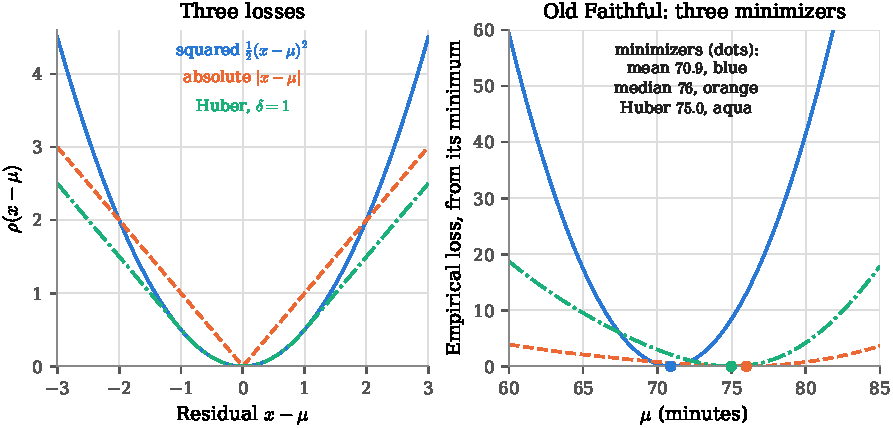
\includegraphics[width=\textwidth]{fig_mestimation_losses}
\caption{Left: the squared (blue), absolute (orange, dashed) and Huber (aqua, dash-dot, $\delta = 1$) losses as functions of the residual. Right: the three empirical losses for the Old Faithful waits, each measured from its minimum, with the minimizers marked.}
\label{fig:mestlosses}
\end{figure}

\begin{proposition}[The median minimizes expected absolute deviation]
\label{prop:median-min}
Let $X$ have $\E\abs{X} < \infty$ and a continuous density $f$, and let $m$ be a median, $\Pr(X < m) = \Pr(X > m) = \frac12$.
Then $Q(\mu) = \E\abs{X - \mu}$ is minimized at $\mu = m$, and at no other point if $f(m) > 0$.
\end{proposition}

\coreproof{The derivative of $Q$ at $\mu$ is the probability below $\mu$ minus the probability above it: each unit you move $\mu$ to the right, the observations below it each cost one more and those above each cost one less. That derivative is negative below the median, zero at it and positive above.}
\begin{proof}
Split the expectation at $\mu$:
\[
Q(\mu) = \int_\mu^\infty (x - \mu)f(x)\,\mathrm{d}x + \int_{-\infty}^\mu (\mu - x)f(x)\,\mathrm{d}x.
\]
Differentiate in $\mu$. The first integral has derivative $-\int_\mu^\infty f(x)\,\mathrm{d}x$ (the integrand's derivative in $\mu$ is $-f$, and the boundary term $(\mu - \mu)f(\mu)$ is $0$); the second has derivative $\int_{-\infty}^\mu f(x)\,\mathrm{d}x$ by the same reasoning \toolkit{sec:math-density}.
So
\[
Q'(\mu) = \Pr(X < \mu) - \Pr(X > \mu) = 2F(\mu) - 1,
\]
where $F$ is the CDF.
This is at most $0$ for $\mu < m$, zero at $m$ and at least $0$ for $\mu > m$, so $Q$ decreases until $m$ and increases after: $m$ is a minimizer. If $f(m) > 0$, then $F$ is strictly increasing near $m$, so $Q'$ is strictly negative just below $m$ and strictly positive just above, and $m$ is the only minimizer (the Laplace and Gaussian densities are positive everywhere, so this applies to them).
\end{proof}

\begin{sanitycheck}[Is the kiss proportion a median too?]
The median of $\Bern(0.645)$ is $1$: more than half the mass sits there.
So the absolute loss, which estimates the median, would estimate `$1$' for the kiss experiment, and indeed the sample median of $80$ ones and $44$ zeros is $1$.
That is correct and useless.
A loss chooses what it estimates (an M-estimator estimates whatever its $Q$ is minimized at), and for a proportion the squared loss, which estimates the mean $p$, is the one that answers the question.
\end{sanitycheck}

\subsection{Asymptotic normality of M-estimators}
\label{sec:mest-normal}

The argument of \cref{ch:mle-properties} used only that the log-likelihood is a sum of i.i.d.\ terms.
Every empirical loss is one, so the argument goes through, with one change: the two roles the Fisher information played, as the variance of the score and as the curvature, are now played by two different numbers.

\begin{definition}[The $J$ and $K$ of a loss]
\label{def:jk}
For a loss $\rho$ twice differentiable in $\mu$, with $\mu \in \real^d$, define
\[
J(\mu) = \E\big[\nabla^2_\mu\,\rho(X, \mu)\big], \qquad K(\mu) = \mathrm{Cov}\big(\nabla_\mu\,\rho(X, \mu)\big),
\]
the expected Hessian of the loss (the curvature of $Q$ at $\mu$) and the covariance matrix of its gradient (as the Fisher information matrix of \cref{def:fisher} is the covariance of the score). For $d = 1$ they are $J(\mu) = \E[\partial^2_\mu\rho(X, \mu)]$ and $K(\mu) = \var(\partial_\mu\rho(X, \mu))$.
\end{definition}

\begin{inwords}
\textbf{In words.} $K$ is how much one observation's push on the estimate varies: the analogue of the variance of the score. $J$ is how hard the expected loss resists being pushed: the analogue of the curvature. For the negative log-likelihood the two coincide and both equal the Fisher information, by \cref{thm:fisher-curvature}; for any other loss they are different numbers.
\par\smallskip
\textbf{For the kiss data.} With the squared loss, $\partial_\mu\rho = -2(R - \mu)$ and $\partial^2_\mu\rho = 2$, so $J = 2$ and $K = 4\var(R) = 4p(1 - p)$: at $p = 0.645$, $K = 0.916$.
\end{inwords}

\recall{\Cref{thm:mle-normal} and its proof: for an estimator defined by $\sum_i g_i'(\hat{\mu}) = 0$, the mean value theorem writes $0 = \sum_i g_i'(\mu^*) + \sum_i g_i''(\tilde{\mu})(\hat{\mu} - \mu^*)$; the CLT handles the first sum, the LLN the second, Slutsky the ratio.}

\begin{theorem}[Asymptotic normality of M-estimators]
\label{thm:mest-normal}
Let $\Xton$ be i.i.d.\ from $\Pr$ and let $\mu^*$ be the unique minimizer of $Q$, in the interior of $\mathcal{M}$ (the analogue of condition 3 of \cref{sec:mle-regularity}).
Suppose the hypotheses of \cref{thm:mle-consistent} hold with $\rho$ in place of $-\log p_\theta$ (a bounded closed $\mathcal{M}$, or the restriction argument given there; $\rho$ continuous in $\mu$; $\E[\sup_\mu\abs{\rho(X, \mu)}] < \infty$), so that $\hat{\mu}_n \convp \mu^*$.
Suppose also that $\rho$ is three times differentiable in $\mu$ near $\mu^*$, that derivatives in $\mu$ can be moved inside $\E$ at $\mu^*$, that $K(\mu^*)$ and $\E[\partial^2_\mu\rho(X, \mu^*)]$ are finite with $J(\mu^*)$ invertible (the analogue of condition 5), and that $\abs{\partial^3_\mu\rho(X, \mu)} \leq B(X)$ near $\mu^*$ for some $B$ with $\E[B(X)] < \infty$ (the analogue of condition 4).
Then
\[
\sqrt{n}\,(\hat{\mu}_n - \mu^*) \convd \Gauss_d\Big(0,\; J(\mu^*)^{-1}K(\mu^*)J(\mu^*)^{-1}\Big).
\]
For $d = 1$ the asymptotic variance is $K(\mu^*)/J(\mu^*)^2$.
\end{theorem}

\optionalproof{Word for word the proof of \cref{thm:mle-normal}, with $\rho$ in place of $-\log p_\theta$. The gradient of the empirical loss is zero at $\hat{\mu}_n$ and, by the CLT, approximately $\Gauss(0, K/n)$ at $\mu^*$ (its mean is zero there because $\mu^*$ minimizes $Q$). The curvature between is about $J$ by the LLN. Displacement is push over resistance: $(\text{sd } \sqrt{K/n})/J$.}
\begin{proof}
Consistency is \cref{thm:mle-consistent} with $-\log p_\theta$ replaced by $\rho$: the proof there used the uniform LLN and the unique minimizer of the limit, and nothing about the likelihood.
For normality, take $d = 1$.
Since $\mu^*$ minimizes $Q$ and is interior, $Q'(\mu^*) = \E[\partial_\mu\rho(X, \mu^*)] = 0$ (differentiating under the expectation, which the regularity conditions allow).
So the terms $\partial_\mu\rho(X_i, \mu^*)$ are i.i.d.\ with mean $0$ and variance $K(\mu^*)$, and the CLT gives $\frac{1}{\sqrt{n}}\sum_i\partial_\mu\rho(X_i, \mu^*) \convd \Gauss(0, K(\mu^*))$.
Since $\hat{\mu}_n$ is interior with probability tending to $1$, $Q_n'(\hat{\mu}_n) = 0$, and the mean value theorem gives a $\tilde{\mu}_n$ between $\hat{\mu}_n$ and $\mu^*$ with
\[
0 = Q_n'(\hat{\mu}_n) = Q_n'(\mu^*) + Q_n''(\tilde{\mu}_n)(\hat{\mu}_n - \mu^*), \qquad\text{so}\qquad \sqrt{n}(\hat{\mu}_n - \mu^*) = -\,\frac{\sqrt{n}\,Q_n'(\mu^*)}{Q_n''(\tilde{\mu}_n)}.
\]
The numerator is $\frac{1}{\sqrt{n}}\sum_i\partial_\mu\rho(X_i, \mu^*)$, which converges in distribution to $\Gauss(0, K)$.
The denominator is $Q_n''(\tilde{\mu}_n) = \frac1n\sum_i\partial^2_\mu\rho(X_i, \tilde{\mu}_n)$. It converges in probability to $J(\mu^*)$ by the LLN at $\mu^*$ and the bound $B$ on the third derivative, used exactly as $K$ was in the proof of \cref{thm:mle-normal}: the difference between the average second derivative at $\tilde{\mu}_n$ and at $\mu^*$ is at most $\bar{B}_n\abs{\hat{\mu}_n - \mu^*}$, an average converging to $\E[B(X)]$ times a quantity converging to $0$.
Slutsky's theorem gives the limit $-\Gauss(0, K)/J = \Gauss(0, K/J^2)$ (the sign is absorbed, since $-Z$ has the same distribution as $Z$).
In $d$ dimensions the denominator is the matrix $J$, inverted, applied to a Gaussian vector of covariance $K$, giving $J^{-1}KJ^{-1}$.
\end{proof}

\begin{intuition}[why the variance has three factors]
For maximum likelihood the push and the resistance were the same number, $I$, and push over resistance gave $\sqrt{I}/I = 1/\sqrt{I}$.
For a general loss they come apart.
The push has standard deviation $\sqrt{K}$; the resistance is $J$; the displacement has standard deviation $\sqrt{K}/J$, and its variance is $K/J^2$.
In matrix form that is $J^{-1}KJ^{-1}$, the curvature inverted on both sides of the push's covariance, which is why it is called the \textbf{sandwich}.
A loss with a stiff $Q$ (large $J$) and a quiet gradient (small $K$) gives a precise estimator.
\end{intuition}

\begin{worked}[the sandwich for the sample mean]
With the squared loss, $J = 2$ and $K = 4\var(X)$, so the asymptotic variance is $4\var(X)/4 = \var(X)$: the CLT for the sample mean, recovered. For the kiss data, $p(1 - p) = 0.229$.
\end{worked}

\begin{worked}[the Laplace median has asymptotic variance $1$]
\label{wk:laplace-median}
Let $\Xton$ have the Laplace density $f(x) = \frac12 e^{-\abs{x - m}}$ of \cref{ex:lik-laplace}, and estimate the center $m$ by the sample median, the M-estimator for $\rho = \abs{x - \mu}$.
The absolute value has a corner, so \cref{def:jk} does not apply directly; the way around is to compute $J$ as the curvature of $Q$ itself.
From the proof of \cref{prop:median-min}, $Q'(\mu) = 2F(\mu) - 1$, so $J = Q''(m) = 2f(m) = 2 \times \frac12 = 1$.
For $K$, $\partial_\mu\abs{X - \mu} = -\mathrm{sign}(X - \mu)$ away from the corner, which is $\pm 1$ with probability $\frac12$ each at $\mu = m$: variance $1$.
So the asymptotic variance is $K/J^2 = 1$.
The sample mean of Laplace data has asymptotic variance $\var(X) = 2$.
The median is twice as precise, and its standard error is $1/\sqrt{n}$ against the mean's $\sqrt{2/n}$.
(That the theorem's conclusion holds despite the corner is a separate argument, which this book does not reproduce; the formula $1/(4f(m)^2)$ for the median's asymptotic variance is standard.)
\end{worked}

\section{Robustness}
\label{sec:mest-robust}

\Cref{fig:robustmeanmedian} runs the sample mean and the sample median side by side on three symmetric distributions, $20{,}000$ samples of $n = 100$ each.
For Gaussian data the mean is the better estimator of the center: its standard deviation is $0.100$ against the median's $0.124$, matching the asymptotic variances $1$ and $\pi/2$ (the median's $1/(4f(0)^2)$ with $f(0) = 1/\sqrt{2\pi}$).
In about $61\%$ of samples the mean lands closer to the truth.
For Laplace data the order reverses, $0.141$ against $0.108$, and the median is closer in $62\%$ of samples. The mean's $0.141$ is exactly the $\sqrt{2/100}$ of the worked example; the median's $0.108$ is still $8\%$ above its asymptotic $1/\sqrt{100} = 0.100$, because the Laplace density has a corner at the center and the median's distribution approaches its Gaussian limit slowly there.
For Cauchy data, with density $f(x) = 1/(\pi(1 + (x - m)^2))$, the mean does not settle at all: its histogram is spread across the whole axis and beyond, with a standard deviation of $72$ over the $20{,}000$ samples, while the median's is $0.158$, close to its asymptotic $(\pi/2)/10 = 0.157$.

\begin{figure}[htbp]
\centering
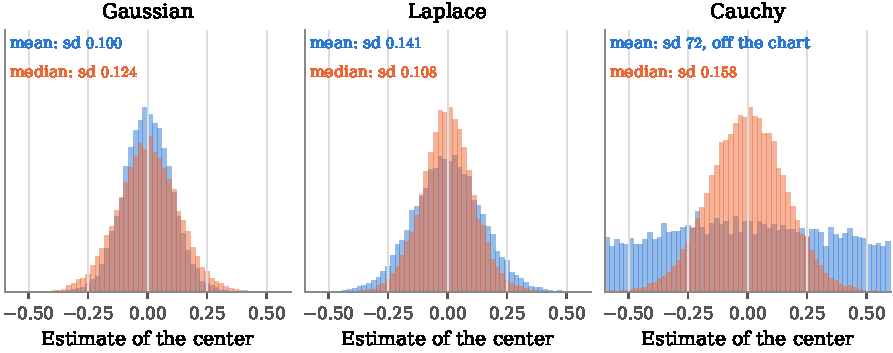
\includegraphics[width=\textwidth]{fig_robust_mean_median}
\caption{The sample mean (blue) and sample median (orange) of $n = 100$ observations, over $20{,}000$ samples, for Gaussian, Laplace and Cauchy data centered at $0$.}
\label{fig:robustmeanmedian}
\end{figure}

\begin{pitfall}[the Cauchy mean]
The Cauchy density has tails so heavy that $\E\abs{X} = \int\abs{x}f(x)\,\mathrm{d}x$ is infinite: the integrand behaves like $1/(\pi\abs{x})$ for large $\abs{x}$, and $\int_1^A \mathrm{d}x/x = \log A \to \infty$.
The mean does not exist, the LLN's hypothesis fails, and the sample mean does not converge to anything.
Worse, the average of $n$ Cauchy observations has exactly the same Cauchy distribution as a single observation: averaging $100$ of them buys nothing.
The method of moments is unavailable (no moments), the sample mean is useless, and the median, the MLE and Huber's estimator all work, with the Cauchy MLE of the center attaining the Cram\'er--Rao variance $2$, against the median's $\pi^2/4 = 2.47$. (Since $\E\abs{X} = \infty$, the absolute loss has infinite expectation here and \cref{def:mest} does not literally apply; the fix is the loss $\abs{x - \mu} - \abs{x}$, which is bounded by $\abs{\mu}$, has finite expectation for every distribution, and has the same minimizer and the same M-estimator, since subtracting $\abs{x}$ shifts $Q_n$ by a constant.)
\end{pitfall}

An estimator that keeps working when the data have heavy tails, or when a few observations are wrong (a decimal point in the wrong place, a sensor fault), is called \textbf{robust}.
The sample median is the simplest robust estimator of a center: move the largest observation to $10^{10}$ and the median does not change, while the mean goes to infinity.
Its price is efficiency on clean Gaussian data, where it is $\pi/2 = 1.57$ times noisier than the mean, so that it needs $57\%$ more observations for the same precision.
Huber's loss is the compromise.

\begin{intuition}[Huber's loss: a mean in the middle, a median in the tails]
$h_\delta(u)$ is $u^2/2$ for $\abs{u} \leq \delta$ and $\delta(\abs{u} - \delta/2)$ beyond, joined so that the function and its slope are continuous (\cref{fig:mestlosses}, left).
Its derivative is the \textbf{clip} function: $u$ inside $[-\delta, \delta]$ and $\pm\delta$ outside.
So an observation within $\delta$ of the current center pushes it the way the squared loss would, in proportion to its distance, and an observation beyond $\delta$ pushes with the fixed force $\delta$, the way the absolute loss would, however far away it is.
A wild observation can push at most $\delta$: that is the robustness.
Observations in the bulk are treated as the mean treats them: that is the efficiency.
The constant $\delta$ sets where `the bulk' ends, and a common choice on data with scale $1$ is $\delta = 1.345$, which costs only $5\%$ in variance on Gaussian data ($1.05$ against the mean's $1$) while capping the influence of any observation.
\end{intuition}

\begin{worked}[Huber on Laplace data]
Take the Laplace center $m$ and $\rho(x, \mu) = h_\delta(x - \mu)$.
Huber's loss is twice differentiable except at $\pm\delta$, so \cref{def:jk} applies (as with the median, the kink means \cref{thm:mest-normal} does not literally cover it, and the standard argument that extends the theorem to this case is not reproduced here): $\partial^2_\mu\rho = \ind(\abs{X - \mu} \leq \delta)$, and
\[
J(m) = \Pr(\abs{X - m} \leq \delta) = \int_{-\delta}^\delta \tfrac12 e^{-\abs{u}}\,\mathrm{d}u = 1 - e^{-\delta}.
\]
The gradient $-\mathrm{clip}_\delta(X - \mu)$ has mean zero at $m$ by symmetry, and
\[
K(m) = \E\big[\mathrm{clip}_\delta(X - m)^2\big] = \int_{-\delta}^\delta u^2\,\tfrac12 e^{-\abs{u}}\,\mathrm{d}u + \delta^2\Pr(\abs{X - m} > \delta) = 2 - e^{-\delta}(2\delta + 2),
\]
the integral by two integrations by parts.
With $\delta = 1$: $J = 0.632$, $K = 0.528$ and the asymptotic variance $K/J^2 = 1.32$, between the median's $1$ and the mean's $2$.
As $\delta \to 0$ the variance tends to $1$ (Huber becomes the median) and as $\delta \to \infty$ it tends to $2$ (Huber becomes the mean); at $\delta = 0.5$ it is $1.17$, at $\delta = 2$ it is $1.59$.
\end{worked}

\begin{bridge}[trimmed means and `robust standard errors']
An introductory course may have mentioned the trimmed mean, the average after discarding the top and bottom $10\%$, as a compromise between mean and median.
Huber's estimator is the principled version: instead of discarding the extremes it caps their influence, and it comes with a standard error, $\sqrt{K/(nJ^2)}$ with $J$ and $K$ estimated from the data.
The sandwich formula also underlies the `robust' or `heteroskedasticity-consistent' standard errors of regression software: least squares is an M-estimator with the squared loss, and when the errors are not identically distributed $K$ is no longer a multiple of $J$, so the usual standard error ($\sigma^2$ times the inverse of $\E[XX^\top]$) is wrong and the sandwich $J^{-1}KJ^{-1}$ is right.
\Cref{ch:regression-multi} returns to this.
\end{bridge}

\section{What comes next}
\label{sec:mom-next}

Part IV is complete: three recipes, each consistent and asymptotically normal, each with a variance you can compute and plug in to get $\text{estimate} \pm 1.96\,\text{standard error}$.
Maximum likelihood has the smallest variance when the model is right; the method of moments is the same estimator for the common families and a fallback when the likelihood is awkward; M-estimation with a robust loss gives up a little precision for protection against heavy tails and bad data.
\Cref{ch:t-test} opens Part V by handling the one situation none of this covers, a small Gaussian sample where the limit theorems have not taken hold, with exact distributions in place of asymptotic ones.
\Cref{ch:wald-lrt} turns the asymptotic normality of \cref{ch:mle-properties} into tests.
\Cref{ch:exp-families} explains why the method of moments and maximum likelihood kept agreeing.

\section{Summary}
\label{sec:mom-summary}

\begin{itemize}[nosep]
\item Method of moments: $\hat{\theta}^{\text{MM}} = M^{-1}(\hat{m}_1, \ldots, \hat{m}_d)$, the parameter whose first $d$ moments match the sample's. Bernoulli, Poisson, exponential and Gaussian all give the MLE; $\Unif([0, \theta])$ gives $2\bar{X}_n$, not the MLE.
\item Its asymptotic variance, by the multivariate CLT and the delta method, is $\nabla M^{-1}\,\Sigma\,(\nabla M^{-1})^\top$; for $d = 1$, $((M^{-1})')^2\var(X)$. It is never below $1/I$. Higher moments make worse estimators ($11/9$ against $1$ for the Poisson rate).
\item M-estimator: $\hat{\mu}_n = \operatorname{argmin}\frac1n\sum_i\rho(X_i, \mu)$ for a loss whose expectation $Q$ is minimized at $\mu^*$. Squared loss gives the mean, absolute loss the median ($Q' = 2F - 1$), check loss the quantile, negative log-likelihood the MLE, Huber's loss a robust center.
\item Asymptotic variance $J^{-1}KJ^{-1}$ with $J = \E[\nabla^2\rho]$ (resistance) and $K = \mathrm{Cov}(\nabla\rho)$ (push); for the MLE $J = K = I$. Laplace median $1$ against mean $2$; Gaussian median $\pi/2$ against mean $1$; Huber with $\delta = 1$ on Laplace data $1.32$.
\item Cauchy data have no mean; the sample mean of $100$ of them is as noisy as one. The median, Huber and the MLE still work.
\end{itemize}

\section{Exercises}
\label{sec:mom-exercises}

\begin{exercise}
\label{ex:mom-gauss-data}
For the four observations $0.5, 1.8, -2.3, 0.9$ from a $\Gauss(\mu, \sigma^2)$ model, compute the method of moments estimates of $\mu$ and $\sigma$.
\end{exercise}
\begin{solution}
$\hat{m}_1 = (0.5 + 1.8 - 2.3 + 0.9)/4 = 0.225$ and $\hat{m}_2 = (0.25 + 3.24 + 5.29 + 0.81)/4 = 2.3975$. So $\hat{\mu} = 0.225$ and $\hat{\sigma} = \sqrt{2.3975 - 0.225^2} = \sqrt{2.347} = 1.532$. These are the MLEs as well; the divide-by-$(n-1)$ sample standard deviation would be $1.532\sqrt{4/3} = 1.769$.
\end{solution}

\begin{exercise}
\label{ex:mom-uniform}
For $\Xton \iid \Unif([0, \theta])$, find the method of moments estimator and its asymptotic variance, and compare its standard deviation at $n = 100$, $\theta = 10$ with the MLE's, whose error is about $\theta/n$ in size (\cref{ex:mle-uniform-rate}).
\end{exercise}
\begin{solution}
$m_1 = \theta/2$, so $\hat{\theta}^{\text{MM}} = 2\bar{X}_n$. With $M^{-1}(m) = 2m$ and $\var(X) = \theta^2/12$, the asymptotic variance is $4\theta^2/12 = \theta^2/3$, and the standard deviation at $n = 100$ is $\sqrt{100/3}/10 = 0.577$. The MLE's error is of order $\theta/n = 0.1$, six times smaller, and shrinking like $1/n$ rather than $1/\sqrt{n}$. The method of moments estimator is unbiased and asymptotically normal, and the MLE beats it anyway: the model is not regular, so the Cram\'er--Rao floor that would protect a regular MLE's variance does not exist here, and the MLE goes below it.
\end{solution}

\begin{exercise}
\label{ex:mom-gamma}
The Gamma family with shape $a > 0$ and rate $b > 0$ has $m_1 = a/b$ and $m_2 = a(a + 1)/b^2$. Find the method of moments estimators of $a$ and $b$. (The MLE of this family has no closed form, which is why the method of moments is used for it.)
\end{exercise}
\begin{solution}
From $m_2 - m_1^2 = a/b^2$ (the variance) and $m_1 = a/b$: dividing, $m_1/(m_2 - m_1^2) = b$, and then $a = m_1 b = m_1^2/(m_2 - m_1^2)$. So $\hat{b} = \hat{m}_1/(\hat{m}_2 - \hat{m}_1^2) = \bar{X}_n/\widehat{\sigma^2}$ and $\hat{a} = \bar{X}_n^2/\widehat{\sigma^2}$, with $\widehat{\sigma^2}$ the divide-by-$n$ sample variance. Two moments, two unknowns, solved in two lines; the likelihood equations involve the derivative of $\log\Gamma(a)$ and need a numerical solver.
\end{solution}

\begin{exercise}
\label{ex:mest-quantile}
Show that $Q(\mu) = \E[C_\alpha(X - \mu)]$, with the check loss $C_\alpha(u) = \alpha u$ for $u \geq 0$ and $-(1 - \alpha)u$ for $u < 0$, is minimized at the $\alpha$-quantile of a continuous $X$ with $\E\abs{X} < \infty$, the point $q$ with $F(q) = \alpha$.
\end{exercise}
\begin{solution}
$Q(\mu) = \alpha\int_\mu^\infty (x - \mu)f(x)\,\mathrm{d}x + (1 - \alpha)\int_{-\infty}^\mu (\mu - x)f(x)\,\mathrm{d}x$. Differentiating as in \cref{prop:median-min}, $Q'(\mu) = -\alpha\Pr(X > \mu) + (1 - \alpha)\Pr(X < \mu) = -\alpha(1 - F(\mu)) + (1 - \alpha)F(\mu) = F(\mu) - \alpha$. This is zero exactly when $F(\mu) = \alpha$, negative below and positive above, so the minimizer is the $\alpha$-quantile. With $\alpha = \frac12$, $Q' = F - \frac12$, half the median's $2F - 1$, and the same minimizer. (The quantile here is the point with probability $\alpha$ \textit{below} it; the book's $q_\alpha$ for Gaussian tails has probability $\alpha$ above, as \cref{ch:gaussian} explains.)
\end{solution}

\begin{exercise}
\label{ex:mest-gauss-median}
For Gaussian data with variance $\sigma^2$, compute the asymptotic variance of the sample median by the $1/(4f(m)^2)$ formula and compare it with the sample mean's. How many more observations does the median need for the same precision?
\end{exercise}
\begin{solution}
$f(m) = 1/(\sigma\sqrt{2\pi})$, so $1/(4f(m)^2) = 2\pi\sigma^2/4 = (\pi/2)\sigma^2 = 1.571\sigma^2$, against $\sigma^2$ for the mean. The median needs $\pi/2 - 1 = 57\%$ more observations. In the simulation of \cref{fig:robustmeanmedian}, $0.124/0.100 = 1.24 \approx \sqrt{\pi/2} = 1.253$.
\end{solution}

\begin{exercise}
\label{ex:mest-huber-gauss}
For Gaussian data with variance $1$ and Huber's loss with $\delta = 1.345$, $J = \Pr(\abs{Z} \leq \delta) = 2\Phi(\delta) - 1$ and $K = \E[\min(Z^2, \delta^2)]$. Given $J = 0.821$ and $K = 0.710$, compute the asymptotic variance and the efficiency relative to the sample mean.
\end{exercise}
\begin{solution}
$K/J^2 = 0.710/0.674 = 1.053$. The mean has asymptotic variance $1$, so Huber's estimator is $5.3\%$ noisier on clean Gaussian data, which is the price of capping every observation's influence at $\delta$. For $\delta = 1$ the figures are $J = 0.683$, $K = 0.516$ and variance $1.107$; for $\delta = 2$, variance $1.010$. The larger $\delta$, the closer to the mean in both efficiency and fragility.
\end{solution}

\begin{exercise}
\label{ex:mest-cauchy-avg}
Accept that the average of $n$ i.i.d.\ Cauchy observations has the same Cauchy distribution as one of them. Explain why this does not contradict the Law of Large Numbers or the Central Limit Theorem, and what it says about $\bar{X}_{1000}$ as an estimate of the center.
\end{exercise}
\begin{solution}
Both theorems assume a finite mean (the LLN as stated in this book assumes a finite variance). The Cauchy has neither: $\int\abs{x}f(x)\,\mathrm{d}x = \infty$. So the theorems say nothing, and the fact is consistent with them. $\bar{X}_{1000}$ is exactly as spread out as a single observation: its probability of landing within $1$ of the center is $\Pr(\abs{X_1 - m} \leq 1) = \frac12$, the same as for $n = 1$. A thousand observations averaged are worth one. The sample median of the same thousand has standard deviation about $\sqrt{\pi^2/4}/\sqrt{1000} = 0.050$.
\end{solution}

\begin{exercise}
\label{ex:mest-sandwich-mle}
Show that for the loss $\rho(x, \theta) = -\log p_\theta(x)$ in a regular model, $J(\theta^*) = K(\theta^*) = I(\theta^*)$, so that \cref{thm:mest-normal} reduces to \cref{thm:mle-normal}.
\end{exercise}
\begin{solution}
$\nabla_\theta\rho = -\nabla_\theta\log p_\theta(X)$, the negative score, whose covariance is the covariance of the score, $I(\theta^*)$ by \cref{def:fisher} (a sign flip does not change a covariance). $\nabla^2_\theta\rho = -\nabla^2_\theta\log p_\theta(X)$, whose expectation is $-\E[\nabla^2\ell] = I(\theta^*)$ by \cref{thm:fisher-curvature}. So $J = K = I$ and $J^{-1}KJ^{-1} = I^{-1}II^{-1} = I^{-1}$.
\end{solution}
